% This file was created with tikzplotlib v0.10.1.
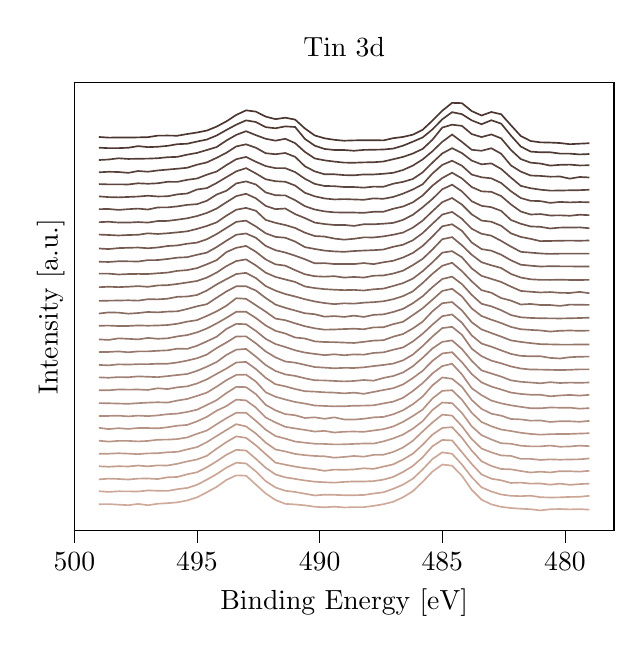
\begin{tikzpicture}

\definecolor{darkgray176}{RGB}{176,176,176}
\definecolor{darkolivegreen1027769}{RGB}{102,77,69}
\definecolor{darkolivegreen836154}{RGB}{83,61,54}
\definecolor{darkolivegreen886558}{RGB}{88,65,58}
\definecolor{darkolivegreen926962}{RGB}{92,69,62}
\definecolor{darkolivegreen977365}{RGB}{97,73,65}
\definecolor{darkslategray745347}{RGB}{74,53,47}
\definecolor{darkslategray795751}{RGB}{79,57,51}
\definecolor{dimgray1068173}{RGB}{106,81,73}
\definecolor{dimgray1118576}{RGB}{111,85,76}
\definecolor{dimgray1158980}{RGB}{115,89,80}
\definecolor{dimgray1209384}{RGB}{120,93,84}
\definecolor{dimgray1259787}{RGB}{125,97,87}
\definecolor{dimgray12910191}{RGB}{129,101,91}
\definecolor{dimgray13410595}{RGB}{134,105,95}
\definecolor{dimgray13810998}{RGB}{138,109,98}
\definecolor{gray143113102}{RGB}{143,113,102}
\definecolor{gray148117106}{RGB}{148,117,106}
\definecolor{gray152121109}{RGB}{152,121,109}
\definecolor{gray157125113}{RGB}{157,125,113}
\definecolor{gray161129117}{RGB}{161,129,117}
\definecolor{rosybrown166133120}{RGB}{166,133,120}
\definecolor{rosybrown171137124}{RGB}{171,137,124}
\definecolor{rosybrown175141128}{RGB}{175,141,128}
\definecolor{rosybrown180145131}{RGB}{180,145,131}
\definecolor{rosybrown184149135}{RGB}{184,149,135}
\definecolor{rosybrown189153139}{RGB}{189,153,139}
\definecolor{rosybrown194157142}{RGB}{194,157,142}
\definecolor{rosybrown198161146}{RGB}{198,161,146}
\definecolor{tan203165150}{RGB}{203,165,150}
\definecolor{tan207169153}{RGB}{207,169,153}

\begin{axis}[
scaled y ticks=manual:{}{\pgfmathparse{#1}},
tick align=outside,
title={Tin 3d},
x dir=reverse,
x grid style={darkgray176},
xlabel={Binding Energy [eV]},
xmin=478, xmax=500,
xtick pos=left,
xtick style={color=black},
y grid style={darkgray176},
ylabel={Intensity [a.u.]},
ymajorticks=false,
ymin=-115505.75, ymax=69398.75,
ytick style={color=black},
yticklabels={}
]
\addplot [semithick, darkslategray745347]
table {%
499 46934
498.6 46662
498.2 46715
497.8 46681
497.4 46758
497 46853
496.6 47475
496.2 47510
495.8 47442
495.4 48146
495 48762
494.6 49565
494.2 51194
493.8 53362
493.4 56015
493 57914
492.6 57388
492.2 55337
491.8 54285
491.4 54872
491 54098
490.6 50433
490.2 47557
489.8 46380
489.4 45750
489 45386
488.6 45528
488.2 45592
487.8 45610
487.4 45518
487 46434
486.6 46942
486.2 47877
485.8 49899
485.4 53683
485 57766
484.6 60994
484.2 60880
483.8 57602
483.4 55788
483 57229
482.6 56300
482.2 51764
481.8 47331
481.4 45268
481 44713
480.6 44620
480.2 44430
479.8 43948
479.4 44161
479 44351
};
\addplot [semithick, darkslategray795751]
table {%
499 42502
498.6 42320
498.2 42334
497.8 42488
497.4 43158
497 42742
496.6 42886
496.2 43264
495.8 43956
495.4 44132
495 45038
494.6 45868
494.2 47524
493.8 49823
493.4 51994
493 53781
492.6 53101
492.2 50979
491.8 50523
491.4 51298
491 51037
490.6 46124
490.2 43346
489.8 41989
489.4 41569
489 41552
488.6 41241
488.2 41592
487.8 41666
487.4 41755
487 42142
486.6 43333
486.2 44996
485.8 46728
485.4 50063
485 54230
484.6 57162
484.2 56332
483.8 53789
483.4 52177
483 53831
482.6 52429
482.2 47506
481.8 42991
481.4 40897
481 40608
480.6 40613
480.2 40079
479.8 40053
479.4 39727
479 39905
};
\addplot [semithick, darkolivegreen836154]
table {%
499 37421
498.6 37640
498.2 38133
497.8 37867
497.4 37941
497 37998
496.6 38163
496.2 38579
495.8 38723
495.4 39637
495 40351
494.6 41546
494.2 42763
493.8 45475
493.4 47784
493 49312
492.6 47682
492.2 46192
491.8 45404
491.4 46177
491 44393
490.6 40759
490.2 38086
489.8 37285
489.4 36770
489 36344
488.6 36301
488.2 36452
487.8 36507
487.4 36805
487 37744
486.6 38708
486.2 40111
485.8 42006
485.4 45804
485 50816
484.6 51988
484.2 51509
483.8 48130
483.4 46891
483 47980
482.6 46360
482.2 41568
481.8 37815
481.4 36342
481 35969
480.6 35125
480.2 35430
479.8 35525
479.4 35186
479 35267
};
\addplot [semithick, darkolivegreen886558]
table {%
499 32352
498.6 32571
498.2 32479
497.8 32126
497.4 32891
497 32602
496.6 33121
496.2 33477
495.8 33830
495.4 34231
495 35489
494.6 36436
494.2 38332
493.8 40413
493.4 43029
493 43906
492.6 42495
492.2 40227
491.8 39820
491.4 40313
491 38744
490.6 34843
490.2 32742
489.8 31545
489.4 31538
489 31203
488.6 31110
488.2 31479
487.8 31466
487.4 31747
487 32152
486.6 33298
486.2 35130
485.8 37661
485.4 41043
485 44946
484.6 47931
484.2 44921
483.8 41635
483.4 41242
483 42278
482.6 40034
482.2 35184
481.8 32649
481.4 31035
481 30863
480.6 30550
480.2 30617
479.8 29738
479.4 30426
479 30225
};
\addplot [semithick, darkolivegreen926962]
table {%
499 27503
498.6 27366
498.2 27383
497.8 27341
497.4 27828
497 27637
496.6 27836
496.2 28433
495.8 28418
495.4 29254
495 29796
494.6 31368
494.2 32674
493.8 35322
493.4 37762
493 38694
492.6 36703
492.2 34929
491.8 34072
491.4 34059
491 32457
490.6 29686
490.2 27583
489.8 26722
489.4 26633
489 26283
488.6 26277
488.2 26028
487.8 26449
487.4 26383
487 27656
486.6 28412
486.2 29604
485.8 32323
485.4 36354
485 40145
484.6 42314
484.2 40289
483.8 37192
483.4 35642
483 36041
482.6 33743
482.2 30170
481.8 26762
481.4 25789
481 25194
480.6 24806
480.2 24832
479.8 24937
479.4 24991
479 25168
};
\addplot [semithick, darkolivegreen977365]
table {%
499 22430
498.6 22122
498.2 22025
497.8 22191
497.4 22359
497 22696
496.6 22395
496.2 22468
495.8 23258
495.4 23610
495 25268
494.6 25820
494.2 27947
493.8 30357
493.4 32741
493 34081
492.6 31879
492.2 29487
491.8 28684
491.4 28454
491 26893
490.6 23904
490.2 22458
489.8 21569
489.4 21163
489 21306
488.6 21165
488.2 21025
487.8 21598
487.4 21427
487 22205
486.6 23559
486.2 25282
485.8 27410
485.4 31883
485 35411
484.6 37133
484.2 35086
483.8 31426
483.4 30310
483 29858
482.6 27949
482.2 24543
481.8 21748
481.4 20600
481 20479
480.6 19732
480.2 20147
479.8 19945
479.4 20089
479 19995
};
\addplot [semithick, darkolivegreen1027769]
table {%
499 17167
498.6 17220
498.2 16852
497.8 17152
497.4 17382
497 17008
496.6 17868
496.2 17888
495.8 18295
495.4 18923
495 19213
494.6 20611
494.2 23169
493.8 24743
493.4 27765
493 28606
492.6 27339
492.2 24069
491.8 22900
491.4 22823
491 20857
490.6 18390
490.2 17015
489.8 16245
489.4 15834
489 15777
488.6 15759
488.2 15637
487.8 16072
487.4 16093
487 17328
486.6 18252
486.2 19970
485.8 22786
485.4 26870
485 30000
484.6 32193
484.2 29834
483.8 26279
483.4 24504
483 24297
482.6 22566
482.2 19102
481.8 16198
481.4 14942
481 15136
480.6 14545
480.2 14613
479.8 14433
479.4 14856
479 14674
};
\addplot [semithick, dimgray1068173]
table {%
499 11783
498.6 11971
498.2 11637
497.8 11623
497.4 11835
497 11616
496.6 12253
496.2 12310
495.8 12806
495.4 13381
495 14311
494.6 15590
494.2 17400
493.8 19999
493.4 22527
493 23500
492.6 21635
492.2 18507
491.8 17165
491.4 17425
491 15125
490.6 13469
490.2 11624
489.8 11017
489.4 10637
489 10656
488.6 10237
488.2 10934
487.8 10926
487.4 11158
487 11498
486.6 12741
486.2 14829
485.8 17927
485.4 21379
485 25361
484.6 27244
484.2 24498
483.8 20425
483.4 18536
483 17965
482.6 16459
482.2 12694
481.8 11129
481.4 10030
481 9866
480.6 9192
480.2 9554
479.8 9582
479.4 9636
479 9284
};
\addplot [semithick, dimgray1118576]
table {%
499 6678
498.6 6508
498.2 6302
497.8 6491
497.4 6593
497 7189
496.6 6923
496.2 7208
495.8 7586
495.4 8018
495 9010
494.6 10225
494.2 11698
493.8 14476
493.4 16918
493 17680
492.6 16502
492.2 12728
491.8 11514
491.4 10603
491 9394
490.6 7465
490.2 6072
489.8 5853
489.4 5025
489 4576
488.6 4941
488.2 5513
487.8 5487
487.4 5930
487 6605
486.6 7506
486.2 9538
485.8 12422
485.4 16305
485 20048
484.6 21764
484.2 19062
483.8 15016
483.4 12457
483 11973
482.6 10296
482.2 7183
481.8 5710
481.4 4911
481 3974
480.6 4041
480.2 4137
479.8 4187
479.4 4130
479 4230
};
\addplot [semithick, dimgray1158980]
table {%
499 937
498.6 696
498.2 1093
497.8 1223
497.4 1329
497 1034
496.6 1353
496.2 1948
495.8 2197
495.4 2904
495 3357
494.6 4733
494.2 6875
493.8 9406
493.4 11915
493 12423
492.6 10018
492.2 7215
491.8 5714
491.4 5370
491 3795
490.6 1503
490.2 738
489.8 70
489.4 -262
489 -440
488.6 -113
488.2 89
487.8 233
487.4 505
487 1640
486.6 2487
486.2 4315
485.8 7294
485.4 11126
485 14924
484.6 16027
484.2 13177
483.8 9067
483.4 7017
483 6203
482.6 4075
482.2 1716
481.8 -439
481.4 -773
481 -1107
480.6 -1300
480.2 -1189
479.8 -1181
479.4 -1202
479 -1175
};
\addplot [semithick, dimgray1209384]
table {%
499 -4545
498.6 -4623
498.2 -4338
497.8 -4363
497.4 -4437
497 -3862
496.6 -3843
496.2 -3395
495.8 -2840
495.4 -2657
495 -1653
494.6 -777
494.2 1502
493.8 4146
493.4 6605
493 7120
492.6 5374
492.2 2004
491.8 230
491.4 -720
491 -2039
490.6 -3506
490.2 -5185
489.8 -5104
489.4 -5482
489 -5440
488.6 -5496
488.2 -5068
487.8 -5522
487.4 -4754
487 -4136
486.6 -2781
486.2 -907
485.8 1993
485.4 5893
485 10086
484.6 10924
484.2 8239
483.8 3389
483.4 687
483 31
482.6 -1635
482.2 -3934
481.8 -5759
481.4 -6154
481 -6497
480.6 -6379
480.2 -6426
479.8 -6449
479.4 -6484
479 -6487
};
\addplot [semithick, dimgray1259787]
table {%
499 -9448
498.6 -9439
498.2 -9788
497.8 -9609
497.4 -9546
497 -9594
496.6 -9286
496.2 -9012
495.8 -8296
495.4 -7980
495 -7160
494.6 -5599
494.2 -3881
493.8 -548
493.4 1205
493 1995
492.6 -416
492.2 -3560
491.8 -5608
491.4 -6144
491 -8000
490.6 -9703
490.2 -10507
489.8 -10692
489.4 -10487
489 -11074
488.6 -10802
488.2 -11059
487.8 -10295
487.4 -10181
487 -9397
486.6 -8213
486.2 -5928
485.8 -3349
485.4 527
485 4761
484.6 5614
484.2 2260
483.8 -1660
483.4 -4725
483 -6001
482.6 -7121
482.2 -9566
481.8 -11045
481.4 -11766
481 -11995
480.6 -12030
480.2 -11925
479.8 -12047
479.4 -12049
479 -12006
};
\addplot [semithick, dimgray12910191]
table {%
499 -15032
498.6 -14842
498.2 -14998
497.8 -14830
497.4 -14583
497 -14880
496.6 -14301
496.2 -14190
495.8 -13704
495.4 -13089
495 -12465
494.6 -11081
494.2 -9007
493.8 -6344
493.4 -4244
493 -3560
492.6 -6042
492.2 -9044
491.8 -10789
491.4 -11847
491 -12855
490.6 -14727
490.2 -15387
489.8 -15825
489.4 -16069
489 -16238
488.6 -16141
488.2 -16399
487.8 -15889
487.4 -15619
487 -14522
486.6 -13343
486.2 -11500
485.8 -8432
485.4 -4764
485 -782
484.6 -149
484.2 -2684
483.8 -7269
483.4 -10352
483 -11598
482.6 -12873
482.2 -14791
481.8 -16563
481.4 -16906
481 -17198
480.6 -17032
480.2 -17347
479.8 -17416
479.4 -16961
479 -17526
};
\addplot [semithick, dimgray13410595]
table {%
499 -20685
498.6 -20586
498.2 -20523
497.8 -20433
497.4 -20579
497 -19989
496.6 -20048
496.2 -19779
495.8 -18993
495.4 -18880
495 -18250
494.6 -16420
494.2 -13901
493.8 -11717
493.4 -9603
493 -9121
492.6 -11268
492.2 -14558
491.8 -16444
491.4 -17855
491 -18862
490.6 -19997
490.2 -20911
489.8 -21566
489.4 -22013
489 -21678
488.6 -21810
488.2 -21412
487.8 -21200
487.4 -20828
487 -19985
486.6 -18712
486.2 -16730
485.8 -13300
485.4 -9487
485 -6196
484.6 -4955
484.2 -8404
483.8 -12629
483.4 -16242
483 -17311
482.6 -19510
482.2 -20557
481.8 -22177
481.4 -21935
481 -22372
480.6 -22386
480.2 -22748
479.8 -22216
479.4 -22273
479 -22330
};
\addplot [semithick, dimgray13810998]
table {%
499 -25893
498.6 -25428
498.2 -25522
497.8 -25955
497.4 -25685
497 -25245
496.6 -25416
496.2 -25095
495.8 -24975
495.4 -24021
495 -22912
494.6 -22046
494.2 -19385
493.8 -16789
493.4 -14661
493 -14643
492.6 -16404
492.2 -19460
491.8 -22202
491.4 -23522
491 -24652
490.6 -25779
490.2 -26169
489.8 -27189
489.4 -26942
489 -27292
488.6 -26760
488.2 -27300
487.8 -26439
487.4 -26239
487 -25248
486.6 -23958
486.2 -21654
485.8 -18764
485.4 -14984
485 -11647
484.6 -10682
484.2 -13745
483.8 -18194
483.4 -21869
483 -22921
482.6 -24497
482.2 -26518
481.8 -27438
481.4 -27705
481 -27846
480.6 -27883
480.2 -27927
479.8 -27839
479.4 -27743
479 -27597
};
\addplot [semithick, gray143113102]
table {%
499 -30943
498.6 -30865
498.2 -31037
497.8 -31017
497.4 -30799
497 -30916
496.6 -30818
496.2 -30629
495.8 -30112
495.4 -29235
495 -28629
494.6 -26896
494.2 -25002
493.8 -22673
493.4 -19590
493 -19825
492.6 -22461
492.2 -25108
491.8 -27985
491.4 -28639
491 -29932
490.6 -31130
490.2 -31988
489.8 -32548
489.4 -32471
489 -32283
488.6 -32162
488.2 -32371
487.8 -31610
487.4 -31552
487 -30265
486.6 -29303
486.2 -26553
485.8 -23723
485.4 -20180
485 -16571
484.6 -15694
484.2 -18800
483.8 -23783
483.4 -26913
483 -28431
482.6 -29808
482.2 -31421
481.8 -32365
481.4 -32638
481 -32869
480.6 -33329
480.2 -33010
479.8 -32888
479.4 -33020
479 -32924
};
\addplot [semithick, gray148117106]
table {%
499 -36555
498.6 -36777
498.2 -36132
497.8 -36324
497.4 -36554
497 -35960
496.6 -36294
496.2 -36119
495.8 -35323
495.4 -34778
495 -33659
494.6 -32076
494.2 -29978
493.8 -27660
493.4 -25180
493 -25162
492.6 -27730
492.2 -30820
491.8 -33031
491.4 -34127
491 -35782
490.6 -36191
490.2 -37378
489.8 -37641
489.4 -37702
489 -37873
488.6 -38034
488.2 -37567
487.8 -37060
487.4 -36896
487 -35452
486.6 -34342
486.2 -32042
485.8 -29242
485.4 -24966
485 -21641
484.6 -21155
484.2 -24574
483.8 -29485
483.4 -32433
483 -33938
482.6 -35412
482.2 -36972
481.8 -37600
481.4 -38087
481 -38516
480.6 -38612
480.2 -38705
479.8 -38723
479.4 -38645
479 -38686
};
\addplot [semithick, gray152121109]
table {%
499 -41794
498.6 -41734
498.2 -41514
497.8 -41869
497.4 -41508
497 -41506
496.6 -41246
496.2 -41067
495.8 -40384
495.4 -40480
495 -39182
494.6 -37375
494.2 -35478
493.8 -32250
493.4 -30145
493 -30310
492.6 -33048
492.2 -36338
491.8 -38470
491.4 -39698
491 -41050
490.6 -41998
490.2 -42547
489.8 -43059
489.4 -42699
489 -43092
488.6 -42740
488.2 -42863
487.8 -42157
487.4 -41902
487 -40831
486.6 -39871
486.2 -37422
485.8 -34230
485.4 -30461
485 -26987
484.6 -26276
484.2 -29675
483.8 -34916
483.4 -38273
483 -39566
482.6 -41071
482.2 -42549
481.8 -43349
481.4 -43536
481 -43516
480.6 -44186
480.2 -44433
479.8 -43906
479.4 -43713
479 -43646
};
\addplot [semithick, gray157125113]
table {%
499 -47075
498.6 -47274
498.2 -46838
497.8 -46939
497.4 -46773
497 -46776
496.6 -46594
496.2 -46594
495.8 -46088
495.4 -45303
495 -44341
494.6 -42839
494.2 -40148
493.8 -37842
493.4 -35342
493 -35323
492.6 -38162
492.2 -41529
491.8 -43964
491.4 -45687
491 -46144
490.6 -47054
490.2 -47964
489.8 -48201
489.4 -48483
489 -48292
488.6 -48349
488.2 -48076
487.8 -47562
487.4 -47113
487 -46533
486.6 -45202
486.2 -42838
485.8 -39303
485.4 -35373
485 -31891
484.6 -31384
484.2 -34646
483.8 -40383
483.4 -43475
483 -45306
482.6 -46429
482.2 -47711
481.8 -48569
481.4 -48986
481 -49016
480.6 -49113
480.2 -49208
479.8 -49109
479.4 -48911
479 -48918
};
\addplot [semithick, gray161129117]
table {%
499 -52214
498.6 -52374
498.2 -52105
497.8 -52166
497.4 -51811
497 -51968
496.6 -52127
496.2 -51717
495.8 -51248
495.4 -50842
495 -49538
494.6 -47826
494.2 -45899
493.8 -42976
493.4 -40795
493 -40493
492.6 -43653
492.2 -47128
491.8 -49583
491.4 -51002
491 -51606
490.6 -52601
490.2 -53412
489.8 -53488
489.4 -53699
489 -53878
488.6 -53716
488.2 -53304
487.8 -53598
487.4 -52460
487 -51664
486.6 -50202
486.2 -47638
485.8 -44146
485.4 -40295
485 -37575
484.6 -36973
484.2 -40514
483.8 -45404
483.4 -49328
483 -50616
482.6 -51911
482.2 -53444
481.8 -54043
481.4 -54340
481 -54660
480.6 -54199
480.2 -54550
479.8 -54377
479.4 -54463
479 -54340
};
\addplot [semithick, rosybrown166133120]
table {%
499 -57538
498.6 -57564
498.2 -57188
497.8 -57283
497.4 -57231
497 -57408
496.6 -56719
496.2 -57045
495.8 -56326
495.4 -55928
495 -54740
494.6 -53056
494.2 -50800
493.8 -48589
493.4 -46086
493 -45856
492.6 -48768
492.2 -52404
491.8 -55054
491.4 -55914
491 -57026
490.6 -57923
490.2 -58096
489.8 -58388
489.4 -58509
489 -58826
488.6 -58517
488.2 -59007
487.8 -58227
487.4 -57443
487 -56696
486.6 -55132
486.2 -52514
485.8 -49511
485.4 -45416
485 -42360
484.6 -41844
484.2 -45948
483.8 -50859
483.4 -54280
483 -56012
482.6 -57218
482.2 -58494
481.8 -59057
481.4 -59381
481 -59396
480.6 -60031
480.2 -59688
479.8 -59457
479.4 -59754
479 -59404
};
\addplot [semithick, rosybrown171137124]
table {%
499 -62833
498.6 -62906
498.2 -63024
497.8 -63123
497.4 -62852
497 -62633
496.6 -62493
496.2 -62617
495.8 -61788
495.4 -61127
495 -59878
494.6 -58530
494.2 -56063
493.8 -53370
493.4 -51212
493 -51091
492.6 -53957
492.2 -58350
491.8 -60212
491.4 -61355
491 -62368
490.6 -63026
490.2 -63824
489.8 -64014
489.4 -64171
489 -64137
488.6 -63923
488.2 -63880
487.8 -63742
487.4 -62965
487 -62234
486.6 -60656
486.2 -57850
485.8 -54602
485.4 -50588
485 -47569
484.6 -46602
484.2 -50980
483.8 -56679
483.4 -59555
483 -61773
482.6 -62936
482.2 -63743
481.8 -64377
481.4 -64939
481 -64977
480.6 -64647
480.2 -64739
479.8 -64728
479.4 -65137
479 -64914
};
\addplot [semithick, rosybrown175141128]
table {%
499 -68162
498.6 -68124
498.2 -68011
497.8 -68316
497.4 -67988
497 -68203
496.6 -67904
496.2 -67406
495.8 -67168
495.4 -66478
495 -65570
494.6 -63622
494.2 -61630
493.8 -58686
493.4 -56144
493 -56242
492.6 -59127
492.2 -63534
491.8 -65827
491.4 -67381
491 -67832
490.6 -68973
490.2 -68699
489.8 -69316
489.4 -68710
489 -69584
488.6 -69633
488.2 -69294
487.8 -68718
487.4 -68532
487 -67449
486.6 -65794
486.2 -63314
485.8 -60131
485.4 -55506
485 -52257
484.6 -52800
484.2 -56068
483.8 -61540
483.4 -65205
483 -67196
482.6 -68007
482.2 -69387
481.8 -69551
481.4 -70082
481 -69991
480.6 -70609
480.2 -70321
479.8 -70330
479.4 -70533
479 -70170
};
\addplot [semithick, rosybrown180145131]
table {%
499 -73024
498.6 -73553
498.2 -73186
497.8 -73482
497.4 -73120
497 -73118
496.6 -73243
496.2 -72795
495.8 -72154
495.4 -71836
495 -70360
494.6 -68522
494.2 -65967
493.8 -64069
493.4 -61392
493 -61725
492.6 -64663
492.2 -68775
491.8 -70815
491.4 -72622
491 -73281
490.6 -73897
490.2 -74566
489.8 -74279
489.4 -74978
489 -74639
488.6 -74550
488.2 -74684
487.8 -74129
487.4 -73588
487 -72481
486.6 -70577
486.2 -68181
485.8 -65508
485.4 -60913
485 -57779
484.6 -57522
484.2 -61423
483.8 -66834
483.4 -70621
483 -72380
482.6 -73731
482.2 -74354
481.8 -75066
481.4 -75548
481 -75852
480.6 -75655
480.2 -75573
479.8 -75549
479.4 -75391
479 -75259
};
\addplot [semithick, rosybrown184149135]
table {%
499 -78323
498.6 -78724
498.2 -78421
497.8 -78414
497.4 -78638
497 -78445
496.6 -77934
496.2 -77896
495.8 -77660
495.4 -77007
495 -75500
494.6 -74178
494.2 -71564
493.8 -69078
493.4 -66805
493 -66805
492.6 -70150
492.2 -73800
491.8 -76420
491.4 -77478
491 -78686
490.6 -79158
490.2 -79608
489.8 -79677
489.4 -79868
489 -79832
488.6 -79661
488.2 -79502
487.8 -79534
487.4 -78625
487 -77404
486.6 -75821
486.2 -73388
485.8 -70282
485.4 -65656
485 -62603
484.6 -62859
484.2 -66878
483.8 -72407
483.4 -76040
483 -77843
482.6 -79380
482.2 -79604
481.8 -80405
481.4 -80687
481 -80681
480.6 -80348
480.2 -80828
479.8 -80725
479.4 -80375
479 -80594
};
\addplot [semithick, rosybrown189153139]
table {%
499 -83764
498.6 -83698
498.2 -83520
497.8 -83679
497.4 -83878
497 -83570
496.6 -83509
496.2 -83116
495.8 -82935
495.4 -81931
495 -80979
494.6 -78942
494.2 -76423
493.8 -73944
493.4 -71523
493 -72453
492.6 -75376
492.2 -79128
491.8 -81953
491.4 -82779
491 -83802
490.6 -84297
490.2 -84638
489.8 -84788
489.4 -85344
489 -85047
488.6 -84637
488.2 -84933
487.8 -84195
487.4 -84131
487 -82977
486.6 -81145
486.2 -78383
485.8 -74535
485.4 -70815
485 -67592
484.6 -67993
484.2 -72345
483.8 -77673
483.4 -81569
483 -83138
482.6 -84406
482.2 -84608
481.8 -85844
481.4 -85836
481 -86286
480.6 -86032
480.2 -86183
479.8 -86096
479.4 -86012
479 -85665
};
\addplot [semithick, rosybrown194157142]
table {%
499 -88896
498.6 -89076
498.2 -88875
497.8 -88977
497.4 -88581
497 -88925
496.6 -88518
496.2 -88562
495.8 -87854
495.4 -86904
495 -86086
494.6 -84601
494.2 -81646
493.8 -78923
493.4 -76555
493 -77159
492.6 -80221
492.2 -83862
491.8 -87399
491.4 -88230
491 -89029
490.6 -89654
490.2 -90053
489.8 -90780
489.4 -90265
489 -90347
488.6 -90183
488.2 -89721
487.8 -89966
487.4 -89026
487 -88103
486.6 -86117
486.2 -83707
485.8 -80021
485.4 -75830
485 -73095
484.6 -72753
484.2 -77109
483.8 -82422
483.4 -86813
483 -88756
482.6 -90005
482.2 -90155
481.8 -90841
481.4 -91458
481 -91111
480.6 -91430
480.2 -90908
479.8 -90932
479.4 -91111
479 -90744
};
\addplot [semithick, rosybrown198161146]
table {%
499 -94303
498.6 -93984
498.2 -94126
497.8 -94351
497.4 -93980
497 -93934
496.6 -94161
496.2 -93444
495.8 -93301
495.4 -92191
495 -91365
494.6 -89306
494.2 -86858
493.8 -84146
493.4 -82113
493 -82383
492.6 -85798
492.2 -89507
491.8 -92257
491.4 -93461
491 -94098
490.6 -94754
490.2 -95243
489.8 -95481
489.4 -95645
489 -95341
488.6 -95133
488.2 -95175
487.8 -94995
487.4 -94399
487 -93288
486.6 -91251
486.2 -88759
485.8 -85193
485.4 -80610
485 -78015
484.6 -78241
484.2 -83062
483.8 -87953
483.4 -92257
483 -94006
482.6 -94681
482.2 -95774
481.8 -95619
481.4 -96057
481 -95980
480.6 -96486
480.2 -96045
479.8 -96555
479.4 -96238
479 -96055
};
\addplot [semithick, tan203165150]
table {%
499 -99181
498.6 -99459
498.2 -99218
497.8 -99242
497.4 -99308
497 -98865
496.6 -98976
496.2 -99046
495.8 -98333
495.4 -97841
495 -96537
494.6 -94431
494.2 -92117
493.8 -89452
493.4 -87423
493 -87721
492.6 -90989
492.2 -95002
491.8 -97625
491.4 -98990
491 -99474
490.6 -100215
490.2 -100930
489.8 -100617
489.4 -100669
489 -100827
488.6 -100822
488.2 -100724
487.8 -100129
487.4 -99615
487 -98203
486.6 -96448
486.2 -94020
485.8 -90215
485.4 -85879
485 -83150
484.6 -83730
484.2 -88164
483.8 -93360
483.4 -97568
483 -99302
482.6 -100537
482.2 -101063
481.8 -101215
481.4 -101018
481 -101659
480.6 -101763
480.2 -101703
479.8 -101525
479.4 -101477
479 -101068
};
\addplot [semithick, tan207169153]
table {%
499 -104540
498.6 -104481
498.2 -104724
497.8 -104937
497.4 -104411
497 -104952
496.6 -104341
496.2 -104112
495.8 -103768
495.4 -102975
495 -101710
494.6 -99641
494.2 -97406
493.8 -94513
493.4 -92636
493 -92772
492.6 -96429
492.2 -100097
491.8 -102788
491.4 -104388
491 -104635
490.6 -105002
490.2 -105580
489.8 -105824
489.4 -105553
489 -105872
488.6 -105752
488.2 -105742
487.8 -105215
487.4 -104542
487 -103525
486.6 -101672
486.2 -99181
485.8 -95311
485.4 -91070
485 -88176
484.6 -88634
484.2 -92795
483.8 -98594
483.4 -102674
483 -104591
482.6 -105622
482.2 -106117
481.8 -106402
481.4 -106595
481 -107101
480.6 -106605
480.2 -106519
479.8 -106677
479.4 -106565
479 -106789
};
\end{axis}

\end{tikzpicture}
